\documentclass[11pt]{article}
\usepackage[a4paper,margin=1in]{geometry}
\usepackage{amsmath,amssymb}
\usepackage{amsthm}
\theoremstyle{definition}
\newtheorem{theorem}{Theorem}
\newtheorem{proposition}{Proposition}
\newtheorem{corollary}{Corollary}
\newtheorem{remark}{Remark}
\newtheorem{example}{Example}
\newtheorem{definition}{Definition}
\usepackage{graphicx}
\usepackage{booktabs,array,calc}
\usepackage[font=small,labelfont=bf]{caption}
\usepackage[colorlinks=true]{hyperref}
\providecommand{\tightlist}{\setlength{\itemsep}{0pt}\setlength{\parskip}{0pt}}
\setcounter{secnumdepth}{-1}
\emergencystretch=3em

\begin{document}

\title{Supplementary Material: An Obstruction Calculus for Viability under Incomplete Observation}
\author{Amin Abaee}
\maketitle

This supplement collects the material condensed from the main text: the complete proofs (S1), the expanded sufficiency review (S2), the bounded constructions and scope remarks (S3), and three additional figures (S4). Notation and numbering follow the main text.

\section*{S1. Complete proofs}

\begin{theorem}[finite-time exit certificate]\label{thm:exit}

Let \(q : X \to \mathbb{R}\) be a constraint function of class \(C^1\) --- the class assumed throughout the exit theorems --- with
\(\mathcal{V} \subseteq \{ q \ge 0 \}\), and suppose the following
hypotheses hold.

(H1.1) There exist constants \(a > 0\) and \(\varepsilon > 0\) such that
on the strip \(\mathcal{S}_a = \{ x : 0 \le q(x) \le a \}\),
\[\sup_{u \in U(x)} \inf_{d \in D(x)} D^+ q(x; f(x,u,d)) \;\le\; -\varepsilon \qquad \forall x \in \mathcal{S}_a, \tag{1}\]
where \(D^+ q(x; v) = \limsup_{h \downarrow 0} [q(x + hv) - q(x)]/h\) is
the upper right Dini derivative of \(q\) in direction \(v\) (for \(C^1\)
\(q\), \(D^+ q(x; v) = \nabla q(x) \cdot v\) --- the form the proof
uses).

(H1.2) \textbf{Closed-loop existence of the adverse realization.} The
disturbance correspondence is lower semicontinuous, or constant, on the
strip, so that the state-dependent adverse selection constructed in the
proof is realized by an admissible control--disturbance pair for which
the Carath\'eodory existence theorem applies. (Alternatively, without (H1.2), the certificate is read against the convexified (relaxed) inclusion
\(\dot x \in \mathrm{co}\, f(x, u(t), D_{\varepsilon}(x, u(t)))\), which
admits solutions under Marchaud-type conditions and preserves the drift
inequality because the constraint is convex in the velocity; closure and
relaxation are the standard tools for this step.)

Then, under hypotheses (H1.1)--(H1.2), for every
admissible control and every initial state \(x_0 \in \mathcal{S}_a\)
there exists an admissible disturbance realization under which the
trajectory attains \(q(x(t)) < 0\) --- hence leaves
\(\{ q \ge 0 \} \supseteq \mathcal{V}\) --- by every time strictly
larger than \(q(x_0)/\varepsilon\):
\(\inf\{ t : q(x(t)) < 0 \} \le q(x_0)/\varepsilon\), in particular
within time at most \(a/\varepsilon\) (since \(q(x_0) \le a\)).
(Convention, used in both exit theorems: \emph{violation} is the strict
inequality \(q < 0\); at \(q = 0\) the state may still lie on
\(\partial \mathcal{V} \subseteq \mathcal{V}\).)

\end{theorem}

\emph{Proof.} Trajectories of \(\dot x = f(x, u(t), d(t))\) exist in the
Carath\'eodory sense under the standing hypotheses --- \(D\)
compact-valued, \(f\) measurable in \(t\) and continuous in \((x,u,d)\),
linearly bounded --- for every measurable control--disturbance pair. The
adverse realization selected below is \emph{state-dependent}, so its
closed-loop realization is an additional requirement --- the content of (H1.2) (\(D\) lower semicontinuous or constant, or
the convexified reading of its parenthetical); convexity of \(D\) was
not needed for the closure step --- closure and relaxation are the
standard tools for it. Fix an admissible control \(u(\cdot)\). For each
\(x \in \mathcal{S}_a\), condition (1) gives
\(\inf_{d \in D(x)} D^+ q(x; f(x,u(t),d)) \le -\varepsilon\). Define the
adverse-selection correspondence
\[D_{\varepsilon}(x, u) \;=\; \big\{ d \in D(x) : D^+ q(x; f(x,u,d)) \le -\varepsilon \big\},\]
which has nonempty values on \(\mathcal{S}_a\) by (1). For \(q\) of
class \(C^1\) the Dini derivative reduces to
\(\nabla q(x) \cdot f(x,u,d)\), continuous in \((x,u,d)\); with the
closed graph and compact values of \(D\) (Section 2.1),
\(D_{\varepsilon}\) then has closed graph and compact values, and the
measurable-selection theorem (Aubin and Frankowska, 1990, Thm. 8.1.3)
supplies a measurable selection \(d(\cdot)\) with
\(d(t) \in D_{\varepsilon}(x(t), u(t))\) along the trajectory. (The proof is carried out for \(q\) of class \(C^1\), as assumed; the locally Lipschitz case requires a separate comparison argument for almost-everywhere-differentiable arcs and is not treated.) Along the realization
\((u(\cdot), d(\cdot))\) from \(x_0\), the fundamental theorem of
calculus along the absolutely continuous trajectory integrates the
inequality to \[q(x(t)) \;\le\; q(x_0) - \varepsilon t\] as long as
\(x(t)\) remains in \(\mathcal{S}_a\). Hence \(q \le 0\) at a time not
exceeding \(q(x_0)/\varepsilon \le a/\varepsilon\). If the trajectory
has not already left the strip by time \(t^* + \delta\) for some
\(\delta > 0\), the comparison continues to apply and gives
\(q(x(t^* + \delta)) \le q(x_0) - \varepsilon(t^* + \delta) \le -\varepsilon\delta < 0\)
with \(t^* = q(x_0)/\varepsilon\); in either case the trajectory
violates \(\{ q \ge 0 \} \supseteq \mathcal{V}\) before every time
strictly larger than \(q(x_0)/\varepsilon\). The selection
\(d(t) \in D_\varepsilon(x(t), u(t))\) is itself nonanticipative
feedback of the pair \((x, u)\) --- a disturbance strategy in the Isaacs
order, responding to the current state and control without anticipating
future controls --- which is what the certificate requires; no
Elliott--Kalton upgrade to a closed-loop strategy is required for the
stated claim. \ensuremath{\square}

\begin{proposition}[epistemic emptiness by admissibility --- a minimal construction]\label{prop:emptiness}

There exists a system with
\(\mathrm{Viab}(\mathcal{V}; U, \pi_{\mathrm{perf}}) = \mathcal{V} \neq \varnothing\)
such that, for a non-injective observation map \(O\), every admissible
initial information state --- the observation fibres
\(B_0 = O^{-1}(O(S_0))\), \(S_0 \in \mathcal{V}\) --- lies outside
\(\mathrm{ERViab}_{\mathcal{I}}(\mathcal{V})\): the epistemic kernel
over the fibre-induced initial beliefs is empty. The mechanism is \emph{admissibility} rather than a hidden mode: the
state-dependent control set of the construction leaves a single common
action at the merged belief --- one that is outward-drifting at the
boundary state --- so the emptiness is the common-action obstruction
(Theorem~\ref{thm:common-action}'s safety case) at minimal size, produced by the control-set primitive rather than by information; the
hidden-mode instance is Example~\ref{ex:hidden-mode}.

\end{proposition}

\emph{Proof (by construction).} Let \(X = [1,2]\), \(\dot S = u - r(S)\)
with \(r : [1,2] \to \mathbb{R}_{++}\) continuous and \textbf{injective
on \([1,2]\)} (e.g.~\(r(S) = S - 1 + c\), \(c > 0\), strictly
increasing), \(U(S) = \{0, r(S)\}\), \(\mathcal{V} = [1,2]\), and the
constant observation \(O(S) \equiv 0\). Under perfect information, the
state-feedback control \(u = r(S)\) gives \(\dot S = 0\), so every
\(S_0 \in \mathcal{V}\) is viable:
\(\mathrm{Viab}(\mathcal{V}; U, \pi_{\mathrm{perf}}) = \mathcal{V}\).
Under the constant observation, the initial information state is the
fibre \(B_0 = [1,2]\), and the set-membership semantics propagates it:
at time \(t\) the belief is \(B_t = \Phi_t(B_0) \cap \mathcal{V}\), the
image of the initial set under the flow generated by the applied control
--- under a constant observation with no exit observation, this
flow-image coincides with the record-compatibility definition of Section
2.3. The common control set at the initial belief is
\[U^B(B_0) = \bigcap_{S \in [1,2]} \{0, r(S)\} = \{0\},\] because
\(r(S) > 0\) for every \(S\) and, by injectivity on \([1,2]\), no single
control equals \(r(S)\) for all \(S\). An observation-based policy may
select time-varying actions, but robust admissibility requires the
selected action to lie in \(U^B(B_t)\) at every \(t\); the propagated
belief \(B_t\) is nonempty and, while the state remains in \([1,2]\),
\(U^B(B_t) = \{0\}\) by the same computation (the flow of
\(\dot S = -r(S)\) with \(r > 0\) moves \(B_t\) monotonically downward,
preserving the injectivity of \(r\) on the surviving interval). Hence
the policy must hold \(u(t) = 0\) almost everywhere, giving
\(\dot S = -r(S) \le -\min_{[1,2]} r < 0\); every compatible trajectory
exits \(\mathcal{V}\) downward in finite time. The same argument applies
verbatim to any initial fibre, since \(O\) is constant. Hence
\(\mathrm{ERViab}_{\mathcal{I}}(\mathcal{V})\) contains no fibre-induced
initial belief, while beliefs that are singletons (exact prior
knowledge) are not admissible initial states of this observation
structure. The system has no disturbance and no estimation error: the
failure is caused entirely by the non-injectivity of \(O\). \ensuremath{\square}

\begin{theorem}[common-action obstruction]\label{thm:common-action}

Let \(B \subseteq \mathcal{V}\) be an information set of the specified observation structure (the safe-control correspondence
\(\mathcal{R}_{\mathcal{V}}\) is defined on \(\mathcal{V}\), so the
belief is taken inside it). Suppose the following hypotheses hold.

(H3.1) The selected action is held until the next observation (sampled
review: no informative observation arrives before the next action must
be selected, and the policy holds the selected action over the review
interval --- the institutional reading; without a positive dwell time
the instantaneous statement below must be replaced by the tube-safety statement below).

(H3.2) Either the \textbf{common admissible action set} is empty,
\[U^B(B) \;=\; \bigcap_{x \in B} U(x) \;=\; \varnothing, \qquad \text{(admissibility obstruction)}\]
or the \textbf{common safe-action set} is empty while common
admissibility holds,
\[\mathcal{R}_{\mathcal{V}}^B(B) \;:=\; \bigcap_{x \in B} \mathcal{R}_{\mathcal{V}}(x) \;=\; \varnothing \quad \text{with} \quad U^B(B) \neq \varnothing, \tag{2} \qquad \text{(safety obstruction)}\]

(H3.3) \textbf{Closed-loop existence of the local adverse selection
(safety case).} The disturbance correspondence is lower semicontinuous,
or locally constant near the boundary point at which the obstruction
fires, so that the local adverse selection of the proof is realized
along the compatible trajectory; alternatively, the certificate is read
against the convexified (relaxed) inclusion, which preserves the
signed drift (the constraint is convex in the velocity).

Then, under hypotheses (H3.1)--(H3.3),
\(B \notin \mathrm{ERViab}_{\mathcal{I}}(\mathcal{V})\): every
compatible state may be individually robustly viable, and the belief is
nevertheless nonviable, because the state-specific safe actions are
incompatible.

\end{theorem}

\emph{Proof.} Let \(\pi\) be any observation-based policy, and let
\(a = \pi(B)\) be the action it selects at the information set \(B\).

\textbf{Admissibility case.} If \(a \notin U^B(B)\), then for some
compatible state \(x \in B\) the action is inadmissible
(\(a \notin U(x)\)): at that state the selected action is not an
admissible control, so the policy fails outright on the compatible
branch from \(x\) --- an obstruction independent of the safe set.

\textbf{Safety case.} Otherwise \(a \in U^B(B)\). Because
\(\bigcap_{x \in B} \mathcal{R}_{\mathcal{V}}(x) = \varnothing\) while
\(\mathcal{R}_{\mathcal{V}}(x) = U(x)\) at interior points of
\(\mathcal{V}\) (no constraint is active there) and \(a \in U(x)\) for
every \(x \in B\), the emptiness of the intersection must be caused by
the boundary: there is a state
\(\bar x \in B \cap \partial \mathcal{V}\) with
\(a \notin \mathcal{R}_{\mathcal{V}}(\bar x)\). By the defining
inequality of the safe-control correspondence, there are an active
constraint \(j\) (with \(q_j(\bar x) = 0\)) and a disturbance
\(\bar d \in D(\bar x)\) such that
\[\nabla q_j(\bar x) \cdot f(\bar x, a, \bar d) < 0.\] With
\(\eta = - \nabla q_j(\bar x) \cdot f(\bar x, a, \bar d) > 0\), define
the adverse-selection correspondence
\(D_{\eta}(x) = \{ d \in D(x) : \nabla q_j(x) \cdot f(x, a, d) \le -\eta/2 \}\)
on a neighbourhood of \(\bar x\); by continuity of the right-hand side
in \((x,d)\) and the closed graph of \(D\) (Section 2.1), it has
nonempty compact values near \(\bar x\) and admits a measurable local
selection \(d(x)\) with \(d(\bar x) = \bar d\). Let the disturbance
realize this selection on a small initial interval (its closed-loop
realization is hypothesis (H3.3)'s content --- \(D\) lower
semicontinuous or locally constant near \(\bar x\), or the convexified
reading); then along the compatible trajectory from \(\bar x\)
(compatible, since \(\bar x \in B\)), \(q_j\) strictly decreases from
\(q_j(\bar x) = 0\) at rate at least \(\eta/2\), so the trajectory
leaves \(\mathcal{V}\) within the first review period --- before any
informative observation can arrive, whichever action the policy takes.
Since \(\pi\) was arbitrary, no observation-based policy keeps every
compatible trajectory in \(\mathcal{V}\):
\(B \notin \mathrm{ERViab}_{\mathcal{I}}(\mathcal{V})\). \ensuremath{\square}

\begin{proposition}[uniform margin gives a tube obstruction at every review length]\label{prop:uniform-margin}
Let \(B\subseteq\mathcal V\) be a compact information set with
\(U^B(B)\neq\varnothing\), \(f\) and \(\nabla q_j\) continuous, and
suppose there is \(\eta>0\) such that for every \(a\in U^B(B)\) there
exist a boundary state \(x_a\in B\cap\partial\mathcal V\), an active
constraint \(j\) with \(q_j(x_a)=0\), and a disturbance \(d_a\in D(x_a)\)
satisfying
\[\nabla q_j(x_a)\cdot f(x_a,a,d_a) \le -\eta.\]
Under the closed-loop existence convention of
Theorem~\ref{thm:common-action}, the tube-safe action set is then empty
at every review length,
\[\mathcal{A}_{\mathrm{tube}}(B,\Delta)=\varnothing \qquad \forall\,\Delta>0,\]
and hence \(B\notin\mathrm{ERViab}_{\mathcal I}(\mathcal V)\) under
sampled review of any length.
\end{proposition}

\emph{Proof.} Fix \(a\in U^B(B)\) and the triple \((x_a,j,d_a)\). By
continuity of \((x,u,d)\mapsto\nabla q_j(x)\cdot f(x,u,d)\) and the closed
graph of \(D\), the drift inequality holds with margin \(-\eta/2\) on a
neighbourhood of \((x_a,a,d_a)\), and a measurable local selection
\(d(x)\) realizes it. Along the trajectory from \(x_a\) under the held
action \(a\) and this adverse selection,
\(q_j(x(t))\le q_j(x_a)-(\eta/2)\,t=-(\eta/2)\,t<0\) for every small
\(t>0\), so the trajectory leaves \(\mathcal V\) in arbitrarily small
positive time; hence \(\mathrm{Reach}_{[0,\Delta]}(B,a)\not\subseteq\mathcal V\)
for every \(\Delta>0\), i.e.\ \(a\notin\mathcal{A}_{\mathrm{tube}}(B,\Delta)\).
Since \(a\in U^B(B)\) was arbitrary,
\(\mathcal{A}_{\mathrm{tube}}(B,\Delta)=\varnothing\) for every
\(\Delta>0\), and the tube-safety form certifies
\(B\notin\mathrm{ERViab}_{\mathcal I}(\mathcal V)\). \ensuremath{\square}

\begin{proposition}[obstruction ladder]\label{prop:ladder}
Under the standing regularity assumptions and the closed-loop existence
convention of Theorem~\ref{thm:common-action}, the common response sets
of Section 2.4 are nested:
\[\mathcal{A}_{\mathrm{tube}}(B,\Delta) \;\subseteq\; \mathcal{R}_{\mathcal{V}}^B(B) \;\subseteq\; U^B(B) \qquad \forall\,\Delta>0,\]
and emptiness descends the ladder:
\[U^B(B)=\varnothing \;\Longrightarrow\; \mathcal{R}_{\mathcal{V}}^B(B)=\varnothing \;\Longrightarrow\; \mathcal{A}_{\mathrm{tube}}(B,\Delta)=\varnothing \;\Longrightarrow\; B\notin\mathrm{ERViab}_{\mathcal{I}}(\mathcal{V}).\]
\end{proposition}

\emph{Proof.} The second inclusion is by definition, since
\(\mathcal{R}_{\mathcal{V}}(x)\subseteq U(x)\) for every \(x\). For the
first, fix \(a\in\mathcal{A}_{\mathrm{tube}}(B,\Delta)\), \(x\in B\) with
an active constraint \(j\) (\(q_j(x)=0\)), and \(d\in D(x)\). If
\(\nabla q_j(x)\cdot f(x,a,d)<0\), then along the trajectory from \(x\)
under the held action \(a\) and the constant disturbance \(d\),
\(q_j(x(t))=\nabla q_j(x)\cdot f(x,a,d)\,t+o(t)<0\) for all small
\(t>0\), so the trajectory leaves \(\mathcal V\) in arbitrarily small
time, contradicting \(a\in\mathcal{A}_{\mathrm{tube}}(B,\Delta)\). Hence
\(\nabla q_j(x)\cdot f(x,a,d)\ge 0\) for every \(d\in D(x)\) and every
active \(j\), i.e.\ \(a\in\mathcal{R}_{\mathcal{V}}(x)\) for every
\(x\in B\), so \(a\in\mathcal{R}_{\mathcal{V}}^B(B)\). \ensuremath{\square}

\begin{theorem}[delayed-information obstruction]\label{thm:delayed}

Let \(B_0\) be an initial information set. Suppose the following
hypotheses hold.

(H4.1) No informative observation arrives before time
\(T_{\mathrm{obs}} > 0\) --- formally, there are branches that are
\textbf{observation-equivalent on \([0, T_{\mathrm{obs}})\)}: they
produce identical observation records throughout that interval, so the
policy cannot distinguish them before \(T_{\mathrm{obs}}\); between
observations the information set evolves by the set-membership semantics
of Section 2.3.

(H4.2) There exist a constraint function \(q\) of class \(C^1\) (the
class of Theorem~\ref{thm:exit}'s proof) with \(\mathcal{V} \subseteq \{ q \ge 0 \}\)
and a constant \(\varepsilon > 0\) such that, \textbf{for every
open-loop control on the blind window} --- every measurable
\(u(\cdot) : [0, T_{\mathrm{obs}}) \to \bigcup_{x \in B_0} U(x)\), the
class of controls that any observation-based policy realizes before the
first informative observation, where its actions are a fixed function of
time --- there are a compatible initial state \(x^* \in B_0\) attaining
\(q(x^*) = \inf_{x \in B_0} q(x)\) (with \(B_0\) compact and \(q\) lower
semicontinuous; otherwise replace the infimum by \(\inf q + \delta\) for
an arbitrary \(\delta\)-minimizer, let \(\delta \downarrow 0\), and read
the timing bound with \(\inf q + \delta\)) and an admissible disturbance
realization such that, along the realized trajectory from \(x^*\) under
that open-loop control, the record remains compatible and
\[D^+ q(x(t); f(x(t), u(t), d(t))) \;\le\; -\varepsilon \qquad \text{while } q(x(t)) > 0, \tag{3}\]

(H4.3) The timing bound holds:
\[T_{\mathrm{obs}} \;>\; \frac{\inf_{x \in B_0} q(x)}{\varepsilon}. \tag{4}\]

Then, under hypotheses (H4.1)--(H4.3),
\(B_0 \notin \mathrm{ERViab}_{\mathcal{I}}(\mathcal{V})\): information
may be accurate but arrive too late.

\end{theorem}

\emph{Proof.} Fix any observation-based policy. By (H4.1) its actions on
\([0, T_{\mathrm{obs}})\) are a fixed open-loop function of time --- the
record carries no informative observation before \(T_{\mathrm{obs}}\),
so every observation-equivalent branch induces the same actions --- and
(H4.2), applied to that open-loop control, supplies a compatible initial
state \(x^*\) with \(q(x^*) = \inf_{x \in B_0} q(x)\) and an admissible
disturbance realization satisfying (3) along the trajectory from \(x^*\)
under those actions, observation-equivalent on \([0, T_{\mathrm{obs}})\)
to the other compatible branches. For \(q\) of class \(C^1\) --- the
class assumed in (H4.2) --- the fundamental theorem of calculus along
the absolutely continuous trajectory integrates (3) to
\[q(x(t)) \;\le\; q(x^*) - \varepsilon t \;=\; \inf_{x \in B_0} q(x) - \varepsilon t\]
while \(q(x(t)) > 0\), so the trajectory attains the violation
convention of Theorem~\ref{thm:exit} --- the strict inequality \(q(x(t)) < 0\) --- by
every time strictly larger than
\(t^* = \inf_{x \in B_0} q(x) / \varepsilon\) (in particular
\(\inf\{ t : q(x(t)) < 0 \} \le t^*\); the same argument with the
\(\delta\)-minimizer bounds the violation time by
\((\inf q + \delta)/\varepsilon\)), and \(t^*\) by (4) is strictly less
than \(T_{\mathrm{obs}}\) --- the violation is strict and precedes the
first informative observation. Until \(t^*\), the record contains no
informative observation: the violating branch is observation-equivalent
to every other compatible branch before \(T_{\mathrm{obs}}\), so the
policy cannot have altered its action in response to the violation
before it occurs. Since the policy was arbitrary and the violating
realization is compatible with the observation record, no
observation-based policy is robustly viable:
\(B_0 \notin \mathrm{ERViab}_{\mathcal{I}}(\mathcal{V})\). \ensuremath{\square}

\begin{theorem}[finite-horizon soundness and completeness]\label{thm:finite-horizon}
An initial belief \(B_0\) admits an observation-based policy that keeps
every compatible trajectory in \(\mathcal V\) for \(N\) steps if and only
if \(B_0\in\mathcal W_N\).
\end{theorem}

\emph{Proof.} \((\Rightarrow)\) Induction on \(N\). The case \(N=0\) is
\(B_0\subseteq\mathcal V\), i.e.\ \(B_0\in\mathcal W_0\). If a policy is
safe for \(N\) steps, its first action \(a\) is admissible at every
compatible state, so \(a\in U^B(B_0)\); for every possible observation
\(y\), the successor belief \(\mathrm{Post}(B_0,a,y)\) is safe for \(N-1\)
steps under the same policy, so by induction
\(\mathrm{Post}(B_0,a,y)\in\mathcal W_{N-1}\); hence
\(B_0\in\mathrm{Pre}(\mathcal W_{N-1})=\mathcal W_N\).

\((\Leftarrow)\) Backward induction. If \(B_k\in\mathcal W_{N-k} =
\mathrm{Pre}(\mathcal W_{N-k-1})\), choose the witness action
\(a_k\in U^B(B_k)\); after the observation \(y_k\) the successor belief
\(B_{k+1}=\mathrm{Post}(B_k,a_k,y_k)\in\mathcal W_{N-k-1}\), and the
recursion continues. By construction every reachable state over \(N\)
steps lies in \(\mathcal V\). \ensuremath{\square}

\begin{proposition}[observation-fibre criterion]\label{prop:fibre}

An exact certifier
based on \(O\) exists if and only if membership in \(K\) is constant on
every observation fibre:
\[O(z_1) = O(z_2) \;\Longrightarrow\; \big[ z_1 \in K \iff z_2 \in K \big] \qquad \forall z_1, z_2 \in Z, \tag{5}\]
equivalently, \(K = O^{-1}(O(K))\) on the admissible domain.

\end{proposition}

\emph{Proof.} (\(\Rightarrow\)) If \(C\) exists and \(O(z_1) = O(z_2)\),
then \(\mathbf{1}_K(z_1) = C(O(z_1)) = C(O(z_2)) = \mathbf{1}_K(z_2)\),
so membership is fibre-constant.

(\(\Leftarrow\)) If (5) holds, define \(C(y) = \mathbf{1}_K(z)\) for any
\(z \in Z\) with \(O(z) = y\); (5) makes \(C\) well defined on \(O(Z)\)
and exact by construction; extend \(C\) arbitrarily on
\(Y \setminus O(Z)\). A \emph{measurable} exact certifier exists under
the same condition on standard Borel spaces when \(O(K)\) is measurable,
taking \(C = \mathbf{1}_{O(K)}\); measurability is the only additional requirement. \ensuremath{\square}

\begin{corollary}[safety-crossing fibres and the certainly-safe set]\label{cor:certainly-safe} If two admissible states share an observation and lie on opposite
sides of the \emph{same} component safety constraint --- with the safe
set of that certification problem read as the single floor
\(K = \{ q_j \ge 0 \}\); or, in the general form of the hypothesis, one
of the two states lies in \(K\) and the other outside \(K\) --- no exact
observation-only certificate exists. (Crossing one floor of an
intersection \(K = \bigcap_j \{ q_j \ge 0 \}\) does not by itself put
the pair on opposite sides of the intersection --- the state satisfying
floor \(j\) may violate floor \(i\) --- hence the single-floor scoping.)
The largest set of observations that can soundly be labeled safe without
further information is the certainly-safe set
\[\mathcal{Y}_{\mathrm{safe}} \;=\; \big\{ y \in O(Z) : O^{-1}(y) \subseteq K \big\}.\]

\end{corollary}

\emph{Proof.} In the general form (one state in \(K\), one outside), the
fibre violates (5) for that \(K\), so Proposition~\ref{prop:fibre} denies the certifier; in
the single-floor form it violates (5) for the floor's own certification
problem (\(K = \{q_j \ge 0\}\)). On \(\mathcal{Y}_{\mathrm{safe}}\)
every compatible state is safe, so the constant verdict ``safe'' is
sound; outside \(\mathcal{Y}_{\mathrm{safe}}\) some compatible state is
unsafe, so no sound ``safe'' verdict exists there. \ensuremath{\square}

\begin{proposition}[monotonicity of the epistemic kernel]\label{prop:monotone}
The robust epistemic kernel is monotone in its constituents: enlarging
the action sets, reducing the disturbance sets, refining the information
structure, or enlarging the policy class never shrinks the kernel.
Writing \(\mathrm{ERViab}^{\,\cdot}\) for the kernel with the indicated
constituent, \(U_1\subseteq U_2\), \(D_1\subseteq D_2\),
\(\Pi_1\subseteq\Pi_2\), and ``\(\mathcal{I}_1\) refines
\(\mathcal{I}_2\)'' imply respectively
\[\mathrm{ERViab}^{U_1} \subseteq \mathrm{ERViab}^{U_2}, \qquad
\mathrm{ERViab}^{D_2} \subseteq \mathrm{ERViab}^{D_1},\]
\[\mathrm{ERViab}^{\Pi_1} \subseteq \mathrm{ERViab}^{\Pi_2}, \qquad
\mathrm{ERViab}^{\mathcal{I}_2} \subseteq \mathrm{ERViab}^{\mathcal{I}_1}.\]
\end{proposition}

\emph{Proof.} Each inclusion is by restriction: a policy that is viable
under the smaller action sets, the larger disturbance sets, the smaller
policy class, or the coarser information structure remains admissible
and nonanticipative under the corresponding enlargement or refinement,
while the adversary's options are unchanged or reduced, so the same
policy witnesses viability. \ensuremath{\square}

\section*{S2. The sufficiency landscape (full)}

\subsection{5. The Sufficiency Landscape}\label{the-sufficiency-landscape-cited}

The sufficiency results against which the obstruction calculus is
defined are standard; they are stated here for contrast, and proofs
appear in the cited sources.

\textbf{(a) Veliov's output-feedback condition.} Veliov (1993) considers the same problem as Section 3 (a tube in the state space under incomplete and inexact measurement) and gives a sufficient condition for the
existence of an \emph{output-feedback regulation map}: a set-valued
feedback of the measurement under which all trajectories starting from
the graph of the tube remain in it. Under perfect measurement his
condition reduces to the classical viability condition (Haddad, 1981).
The complementarity with this paper is exact: Veliov's theorem certifies
existence; the obstruction calculus certifies nonexistence; a problem that satisfies neither requires a stronger observer or a finer observation structure.

\textbf{(b) The estimation-tube programme.} Cardaliaguet, Quincampoix,
and Saint-Pierre (2007) pass from imperfect information in the
measurement space to perfect information in an estimation space of
\emph{sets} of compatible states: the value functions of the two
problems coincide, and the estimation-space problem admits a
Dini-derivative characterization. The reduction is exact for value
functions; what it does not supply is a \emph{common prescription}. The exact relationship is stated in Section 6.3: carried out under the set-membership semantics, the estimation-space solution propagates the belief under a single control signal, so its controls \emph{are} common controls and joint admissibility is built into the estimation-space problem's own admissibility. Pointwise selections taken without that joint-admissibility check need not be jointly admissible; the common-action obstruction (Theorem~\ref{thm:common-action}) is the certificate that no jointly admissible selection exists at the information state in question.

\textbf{(c) Observer-and-buffer transfer.} When a full-information
feedback exists with a strict inward margin, and an observer supplies
exponentially convergent estimates, output feedback of the estimate
preserves safety on a buffered subset: if \(K_\zeta\) is a compact controlled-invariant subset of the interior of the kernel, the state
feedback \(u = k(x)\) is Lipschitz with constant \(L_k\), the observer satisfies \(\|\hat x(t) - x(t)\| \le M e^{-\lambda t}\|\hat x(0) - x(0)\|\), and
the initial estimation error is small enough that
\(L_k M \|\hat x(0) - x(0)\|\) is absorbed by the margin, then \(K_\zeta\) is viable under output feedback (observer-to-viability
transfer with safety buffer; the standard separation argument of observer-based control (Sontag, 1998)). Similarly, eroded kernels: if \(K\) is robustly
invariant under full-state feedback with a strict inward margin on
\(\partial K\), and estimation and implementation errors are bounded by \(\zeta\), then an eroded set \(K^{-c\zeta}\) is invariant
under output feedback for a sensitivity constant \(c > 0\) (erosion
absorbs the error; see the buffer constructions in the literature cited in Section 1.3). These results bound the sufficiency side: under margins and convergence, output feedback \emph{can} work; the obstruction calculus
of Sections 3--4 states the conditions under which it \emph{cannot}.

\textbf{(d) The linear substitution alternative.} For the finite linear
model in which a resource-typed system must meet a demand vector through specified substitution pathways, exactly one of the following holds
(Farkas, 1902; Gale, 1960): (i) there exists a non-negative pathway
vector \(a \ge 0\) satisfying the linear substitution constraints; or
(ii) there exist multipliers \(\alpha, \beta, \gamma \ge 0\) such that
\[\alpha^\top R + \beta^\top E - \gamma^\top Q \ge 0 \quad\text{componentwise},\qquad \gamma^\top s^{\mathrm{req}} > \alpha^\top x + \beta^\top e.\]
The second statement is a certificate that the specified substitution pathways cannot meet demand within the typed resource and capacity
bounds; writing all constraints as \(Aa \le \rho\), the pair is the Farkas lemma alternative. The multipliers are a separation
certificate, not universal exchange rates: nonlinear, nonconvex,
path-dependent, spatial, or irreversible technologies require their own
feasibility analysis, and an elasticity fitted near one operating point
cannot establish global substitutability. This is the feasibility-side
complement of the observation-side obstructions of Sections 3--4: where
the present paper's certificates bound what \emph{information} can
achieve, the substitution alternative bounds what \emph{material
pathways} can achieve, and the same infeasibility logic --- exhibit the separating multiplier rather than assert impossibility --- applies to both.

\begin{center}\rule{0.5\linewidth}{0.5pt}\end{center}


\section*{S3. Bounded constructions and scope remarks}

\subsection{Appendix A: Bounded Constructions and Scope
Remarks}\label{appendix-a-bounded-constructions-and-scope-remarks}

The bounded constructions below complement the obstruction theorems of Sections 3--4. They are stated in full, together with their scope remarks.

\textbf{A.1 Example (coupling creates viability absent in a factor).}
Take the two-patch logistic system
\(\dot S_i = g_i(S_i) + \kappa\,(S_j - S_i) - h_i, \qquad i, j \in \{1,2\},\ i \ne j,\)
with \(g_i(s) = s(1-s)\), \(\kappa = 0.2\), constraints \(S_i \in [0,1]\) and \(h_i \ge h_{\min,i}\) (harvest floors), and admissible controls the constant harvest vectors \(h = (h_1, h_2)\) with \(h_i \ge 0\). Choose
\((S_1^*, S_2^*) = (0.5, 0.8)\). Define harvest floors by the equilibrium equations: \(h_{\min,1} = g_1(0.5) + 0.2(0.8 - 0.5) = 0.31\); \(h_{\min,2} = g_2(0.8) + 0.2(0.5 - 0.8) = 0.10\). Patch 1 in isolation:
\(\max_s g_1(s) = 0.25 < h_{\min,1} = 0.31\), so patch 1 is not viable
in isolation. Yet the coupled system has the equilibrium \((0.5, 0.8)\)
with \(h = (0.31, 0.10)\) admissible and the stock constraints
satisfied, so its kernel is nonempty. The example is the constructive
counterpart of the emptiness results of Section 3: where the obstruction
theorems certify that no policy works for reasons of information, patch
coupling exhibits the opposite direction --- a jointly viable operating
point that no factor sustains alone.

\textbf{A.2 Counterexample (emptiness despite factorwise viability at
MSY).} Take \(\kappa > 0\), \(C_1 \ne C_2\), \(h_{\min,i} = r_i C_i / 4\) (MSY level), in the same coupled system with \(\phi_i(S_i) := g_i(S_i) - h_{\min,i}\) and growth laws
\(g_i(S) = r_i S (1 - S/C_i)\), so that
\[\phi_i(S_i) = -\frac{r_i}{C_i}\left(S_i - \frac{C_i}{2}\right)^2 \le 0\]
with equality only at \(S_i = C_i/2\), and the constraint set is the box \([C_1/2, \bar S_1] \times [C_2/2, \bar S_2]\). Each isolated system has kernel \([C_i/2, \bar S_i]\) (from \(S_i > C_i/2\) the stock
declines toward \(C_i/2\) asymptotically, never below). For the coupled
system, define the Lyapunov function \(W = S_1 + S_2\); then
\[\dot W = \phi_1(S_1) + \phi_2(S_2) \le 0,\] with equality exactly at
\(p^* = (C_1/2, C_2/2)\), where the flow is nevertheless nonzero:
\(\big(\dot S_1, \dot S_2\big)\big|_{p^*} = \left(\tfrac{\kappa}{2}(C_2 - C_1), \tfrac{\kappa}{2}(C_1 - C_2)\right) \ne 0.\)
Suppose a trajectory remained in the constraint box for all time. Then
\(W\) is non-increasing and bounded below by \((C_1 + C_2)/2\), so
\(W(t) \downarrow W_\infty \ge (C_1 + C_2)/2\); the \(\omega\)-limit set
of the trajectory is nonempty, compact, and invariant, and
\(\dot W \equiv 0\) on it (otherwise \(W\) would keep decreasing along
the set). Hence the \(\omega\)-limit set is contained in \(\{p^*\}\), so
it equals \(\{p^*\}\) and the trajectory converges to \(p^*\). But
convergence to \(p^*\) is impossible: along a trajectory with
\(x(t) \to p^*\) the velocity satisfies
\(\dot x(t) = f(x(t)) \to f(p^*) \ne 0\), so
\(x(t) - p^* \sim (t - t_0) f(p^*)\), contradicting convergence.
Therefore no trajectory remains admissible for all time: the kernel is
empty, and since the box is compact and the vector field smooth, every
trajectory violates the constraint in finite time. Note the logical
order: the emptiness conclusion here rests on the
Lyapunov--\(\omega\)-limit argument, \emph{not} on the absence of an
equilibrium --- absence of equilibria alone does not imply an empty
kernel (periodic and nonstationary viable trajectories are possible in
general), and the two are kept separate. The counterexample is
specific to the MSY parameter choice; for \(H_{\min,i} < r_i C_i / 4\),
equilibria may exist. Together with A.1 it delimits what coupling can
and cannot repair: factorwise nonviability is repairable (A.1), but
factorwise viability at an incompatible operating point is not (A.2).


\section*{S4. Additional figures}

\begin{figure}[htbp]
\centering
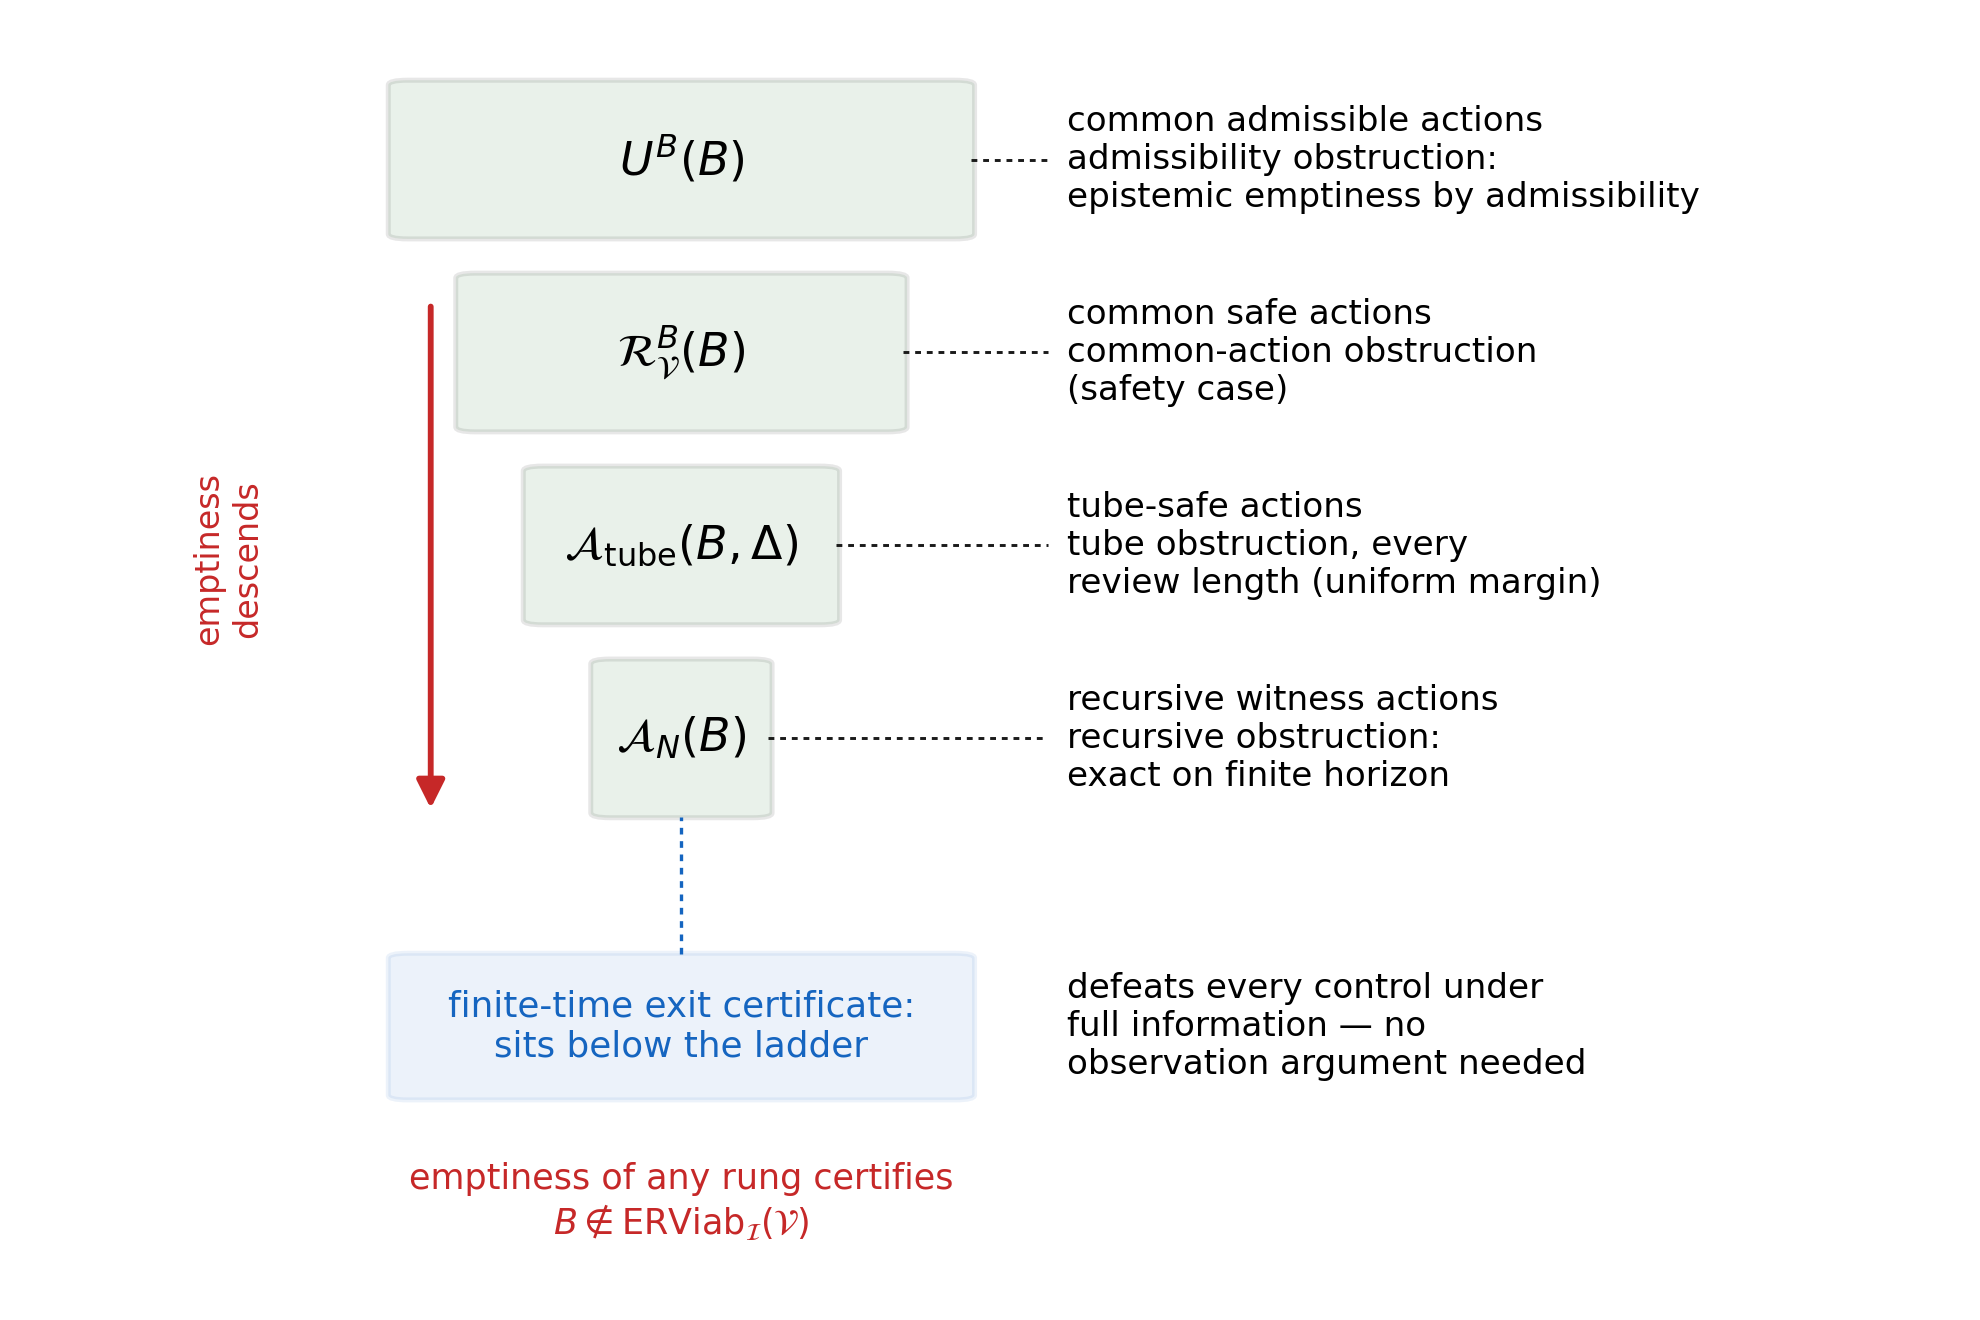
\includegraphics[width=0.75\linewidth]{figs_p2/fig_p2_ladder.png}
\caption{The obstruction ladder. The common response sets are nested,
\(U^B(B)\supseteq\mathcal{R}_{\mathcal{V}}^B(B)\supseteq\mathcal{A}_{\mathrm{tube}}(B,\Delta)\supseteq\mathcal{A}_N(B)\),
and emptiness descends (Proposition~\ref{prop:ladder}); the finite-time
exit certificate sits below the ladder, defeating every control under
full information (Theorem~\ref{thm:exit}).}
\label{fig:ladder}
\end{figure}

\begin{figure}[htbp]
\centering
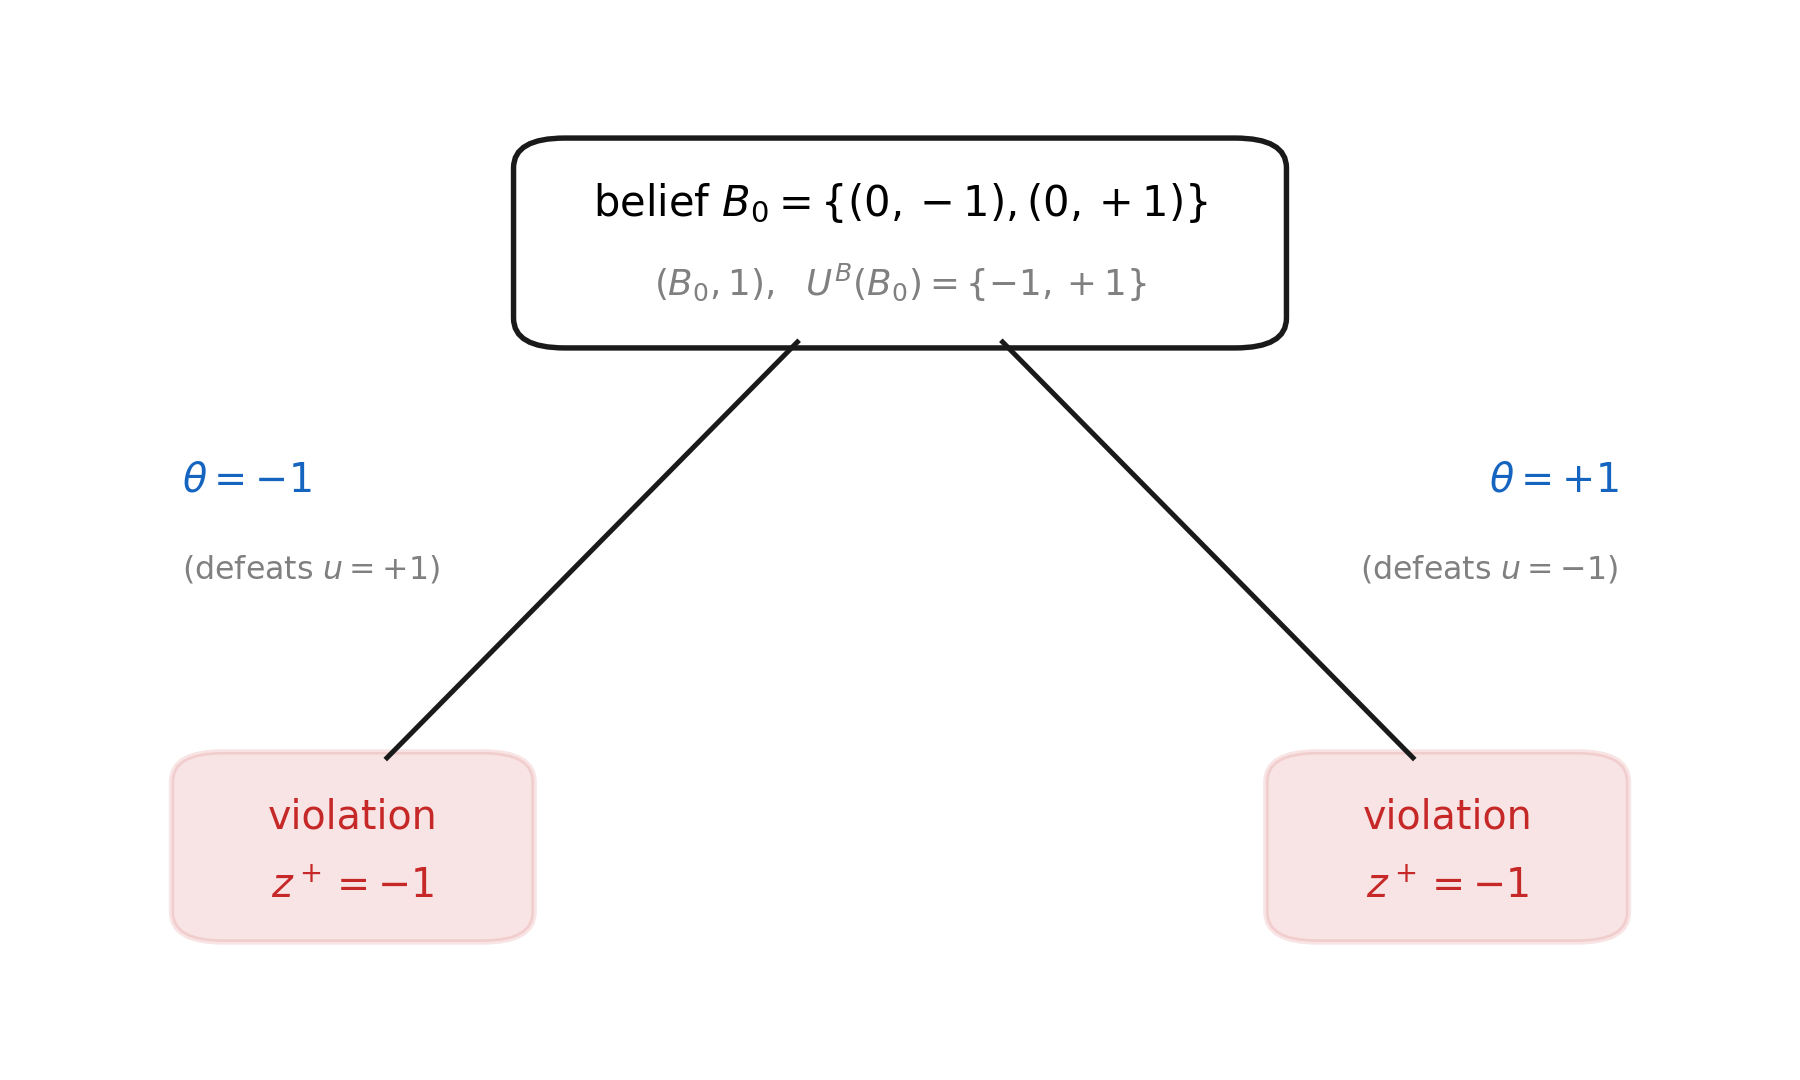
\includegraphics[width=0.66\linewidth]{figs_p2/fig_p2_obstruction_tree.png}
\caption{The one-step obstruction tree of Example~\ref{ex:hidden-mode},
read as a finite system: for each admissible action the adversary has a
compatible branch terminating in violation, so \(B_0\notin\mathcal{W}_1\)
(Theorem~\ref{thm:finite-horizon}).}
\label{fig:obstruction-tree}
\end{figure}

\begin{figure}[htbp]
\centering
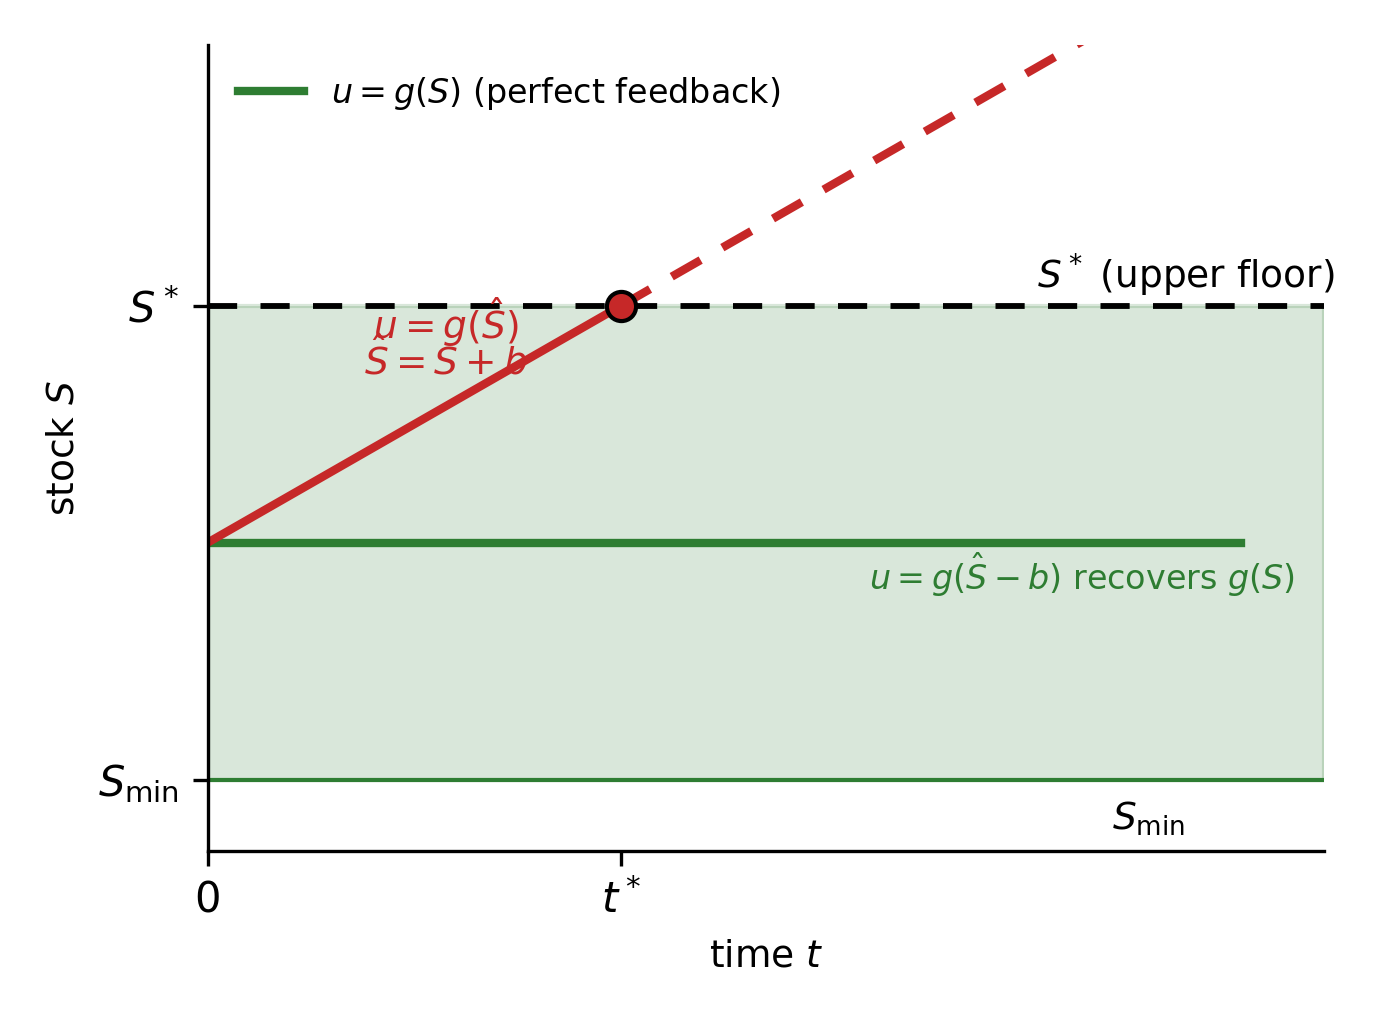
\includegraphics[width=0.62\linewidth]{figs_p2/fig_p2_ce_trap.png}
\caption{The certainty-equivalence trap. Under the perfect-information
law \(u=g(S)\) the stock is stationary inside \(\mathcal V\). Applying
the same law to the biased observation \(u=g(\hat S)\) with
\(\hat S=S+b\) gives \(\dot S=g(S+b)-g(S)>0\), so \(S\) exits above
\(S^*\) in finite time (Remark~\ref{rem:ce-trap}); inverting the bias
restores \(g(S)\).}
\label{fig:ce-trap}
\end{figure}

\section*{Auxiliary definitions and remarks (for reference)}

\begin{definition}[robust epistemic kernel]\label{def:kernel}

\(B_0 \in \mathrm{ERViab}_{\mathcal{I}}(\mathcal{V})\) if there exists a
nonanticipative observation-based policy \(\pi\) such that, for every
compatible initial state \(x_0 \in B_0\) and every admissible
disturbance realization \(d(\cdot)\), the trajectory of
\(\dot x = f(x, u(t), d(t))\) generated from \(x_0\) by \(\pi\)'s
actions under \(d(\cdot)\) --- the record being the one that
\((\pi, d(\cdot))\) generates --- remains in \(\mathcal{V}\) for all
time. (This is the standard exists-strategy-for-all-realizations form. The quantifier order is essential: the record is generated by the realization, so conditioning the admissible realizations on the record would be circular.) Admissible initial
beliefs are the compact information sets \(B_0 \subseteq X\) generated
by the observation structure --- the observation fibres \(O^{-1}(y)\),
\(y \in O(X)\), in the constructions of Sections 3.2--3.4. The existential (non-robust) counterpart \(\mathrm{EViab}_{\mathcal{I}}(\mathcal{V})\) is the non-robust contrast class.

\end{definition}

\begin{proposition}[selector principle]\label{prop:selector}
If \(B\in\mathrm{ERViab}_{\mathcal{I}}(\mathcal{V})\) and \(\pi\) is a
policy witnessing viability on \(B\), then at every review time the
action \(a=\pi(B)\) selected by \(\pi\) is a response that is
(i) \emph{admissible}, \(a\in U^B(B)\); (ii) \emph{safe}, keeping every
compatible trajectory in \(\mathcal{V}\) until the next observation ---
\(\mathrm{Reach}_{[0,\Delta]}(B,a)\subseteq\mathcal{V}\) at review
length \(\Delta\); and (iii) \emph{recursively viable}, in that every
post-observation belief reached at the next review is again in
\(\mathrm{ERViab}_{\mathcal{I}}(\mathcal{V})\) under the continuation
of \(\pi\). A belief is therefore viable only if each of the response
correspondences of this section --- \(U^B(B)\),
\(\mathcal{R}_{\mathcal{V}}^B(B)\), \(\mathcal{A}_{\mathrm{tube}}(B,\Delta)\),
and the recursive predecessor of Section 3.5 --- is nonempty along
every reachable branch; hence a certificate that any one of them is
empty at a reachable belief certifies nonviability. In finite systems
the converse is exact (Theorem~\ref{thm:finite-horizon}); in continuous
time the converse is the backward-recursion completion noted in
Section 6.5.
\end{proposition}

\begin{remark}[comparison-function form]\label{rem:comparison}
Hypothesis (H1.1) uses a constant drift margin \(\varepsilon\). The
certificate extends to state-dependent decline: if there is a continuous
\(\alpha:(0,a]\to(0,\infty)\) with
\[\sup_{u\in U(x)}\inf_{d\in D(x)} D^+q(x; f(x,u,d)) \le -\alpha(q(x)) \qquad \forall x\in\mathcal{S}_a,\]
then the exit-time bound sharpens to
\[t_{\mathrm{exit}} \le \int_0^{q(x_0)} \frac{ds}{\alpha(s)},\]
whenever the integral is finite. The proof replaces the linear comparison
\(q(x(t))\le q(x_0)-\varepsilon t\) with the solution \(r\) of
\(\dot r=-\alpha(r)\), \(r(0)=q(x_0)\), by the standard comparison
argument. If \(\alpha(0)=0\) and the integral diverges, the conclusion
weakens to asymptotic approach rather than finite-time exit; the
constant-margin case \(\alpha\equiv\varepsilon\) is the sharp finite-time
instance.
\end{remark}

\begin{example}[hidden-mode conflict]\label{ex:hidden-mode} Let an unobserved parameter satisfy
\(\theta \in \{-1, +1\}\), with \(\dot z = \theta u\),
\(u \in \{-1, +1\}\), and constraint \(z \ge 0\). At \(z = 0\): if
\(\theta = +1\), only \(u = +1\) is safe; if \(\theta = -1\), only
\(u = -1\) is safe. Both compatible states are individually robustly
viable under full information (each admits its safe control), but the
information set \(B = \{(0, +1), (0, -1)\}\) satisfies
\(\mathcal{R}_{\mathcal{V}}^B(B) = \{+1\} \cap \{-1\} = \varnothing\),
so \(B \notin \mathrm{ERViab}_{\mathcal{I}}(\mathcal{V})\). This is a
purely informational failure: no stochasticity and no estimation-quality
argument is involved. The example is the two-action skeleton of every
``the stock is either recovering or collapsing, and the safe policy
differs between the two'' situation.

\end{example}

\begin{remark}[threshold form of the timing obstruction]\label{rem:sigma}
The delayed-information obstruction has a sharp threshold. Let
\(\sigma^*(B_0)\) be the guaranteed blind-window survival time: the
largest duration such that some pre-observation policy keeps every
observation-equivalent branch in \(\mathcal{V}\) until then,
\[\sigma^*(B_0) \;=\; \sup_{u(\cdot)} \inf_{x_0\in B_0,\, d(\cdot)} \tau(x_0,u,d),\]
with the infimum over branches that remain observation-equivalent on
\([0,T_{\mathrm{obs}})\) and \(\tau\) the first violation time under the
convention of Theorem~\ref{thm:delayed}. Then
\[\sigma^*(B_0) < T_{\mathrm{obs}} \;\Longrightarrow\; B_0 \notin \mathrm{ERViab}_{\mathcal{I}}(\mathcal{V}),\]
because before \(T_{\mathrm{obs}}\) a policy cannot condition its action
on which branch realizes. Condition (4) certifies this threshold: under
(H4.1)--(H4.2) every branch exits by time
\(\inf_{x\in B_0}q(x)/\varepsilon\), hence
\(\sigma^*(B_0)\le\inf_{x\in B_0}q(x)/\varepsilon\), and (4) states that
this upper bound lies below \(T_{\mathrm{obs}}\); the threshold itself
may be strictly smaller, in which case nonviability holds even when (4)
fails. The threshold is the blind-window response correspondence of the
timing layer: its emptiness is the timing certificate, the
delayed-information analogue of the tube and common-action
correspondences.
\end{remark}

\begin{definition}[exact certifier]\label{def:certifier}

For an admissible domain
\(Z \subseteq X\) and a safe set \(K \subseteq Z\), an \textbf{exact
certifier} based on the observation map \(O : Z \to Y\) is a function
\(C : Y \to \{0,1\}\) such that
\[C(O(z)) = 1 \iff z \in K \qquad \text{for every } z \in Z.\]

\end{definition}

\begin{remark}[certainty-equivalence obstruction]\label{rem:ce-trap}

Consider
\(\dot S = u - g(S)\) with \(u \in [0, \bar u]\), \(g\) strictly
increasing on \([S_{\min}, S^* + b]\), \(g(0) = 0\), and
\(\mathcal{V} = [S_{\min}, S^*]\). Assume the range condition
\(g(S + b) \le \bar u\) for every \(S \in [S_{\min}, S^*]\), so that the
certainty-equivalence command below is admissible rather than
inadmissible. Under perfect information the feedback \(u(t) = g(S(t))\)
gives \(\dot S = 0\), so every \(S_0 \in \mathcal{V}\) is viable and
\(\mathrm{Viab}(\mathcal{V}; U, \pi_{\mathrm{perf}}) = \mathcal{V} \neq \varnothing\).
Now take the injective, biased observation \(\hat S = S + b\) with
\(b > 0\), and restrict the policy class to the
\textbf{certainty-equivalence class} \(\Pi_{\mathrm{CE}}\), defined as the class of causal controllers obtained by taking a fixed \emph{perfect-information
regulation law} \(k\) of the plant and applying it directly to the
uncorrected observation, \(u = k(\hat S)\) --- no use of the observation
map's structure (here, the bias \(b\)) enters the law. The trap below is
the member \(k = g\): \(u = g(\hat S)\). Then
\[\dot S = g(S + b) - g(S) > 0 \qquad \forall S,\] and since \(g\) is
strictly increasing on the compact interval \([S_{\min}, S^* + b]\),
\(\dot S\) is bounded below by a positive constant there; hence \(S\)
strictly increases and exits above \(S^*\) in finite time from every
\(S_0 \in \mathcal{V}\):
\[\mathrm{Viab}(\mathcal{V}; U, \Pi_{\mathrm{CE}}) = \varnothing.\] The
mechanism is a \emph{restriction of the policy class}, not a loss of
information: for a known invertible observation the output-feedback
class is as powerful as the state-feedback class,
\(\Pi_{\mathrm{CE}} \subsetneq \Pi_{\mathrm{output}} \cong \Pi_{\mathrm{state}}\),
so
\(\mathrm{Viab}(\mathcal{V}; U, \Pi_{\mathrm{CE}}) \subsetneq \mathrm{Viab}(\mathcal{V}; U, \Pi_{\mathrm{output}}) = \mathrm{Viab}(\mathcal{V}; U, \Pi_{\mathrm{state}})\)
--- the kernel empties exactly when the controller does not apply the correction. An observer who inverts the bias,
\(u = g(\hat S - b) = g(S)\), recovers the perfect-information kernel
--- and lies outside \(\Pi_{\mathrm{CE}}\), since the composite law
\(g(\cdot - b)\) is not a perfect-information law of the plant applied
uncorrected. The remark is the mechanism behind the monitoring-design
consequence of Section 6.4: monitoring bounds observation error so that
a desired state-feedback law is implementable, but the bound is useful
only if the controller uses the correction; an uncorrected biased
indicator empties the kernel that a corrected one preserves. The
phenomenon is the viability-theoretic analogue of Witsenhausen's
counterexample in stochastic control (Witsenhausen, 1968): the
information pattern --- not the dynamics and not the constraint ---
defeats the restricted controller class.

\end{remark}

\subsection{References}\label{references}

\subsection{References}\label{references}

Abaee, A.: The limits of compensatory aggregation: a formal separation of weak and strong sustainability assessment. Zenodo. https://doi.org/10.5281/zenodo.22545740 (2026).

Aubin, J.-P.: Viability Theory. Birkh\"auser, Boston (1991)

Aubin, J.-P.: Viability kernels and capture basins of sets under differential inclusions. SIAM J. Control Optim. \textbf{40}(3), 853--871 (2001)

Aubin, J.-P., Bayen, A.M., Saint-Pierre, P.: Viability Theory: New Directions, 2nd edn. Birkh\"auser, Boston (2011)

Aubin, J.-P., Catt\'e, F.: Bilateral fixed-points and algebraic properties of viability kernels and capture basins of sets. Set-Valued Anal. \textbf{10}, 379--416 (2002)

Aubin, J.-P., Frankowska, H.: Set-Valued Analysis. Birkh\"auser, Boston (1990)

B\'en\'e, C., Doyen, L., Gabay, D.: A viability analysis for a bio-economic
model. Ecol. Econ. \textbf{36}, 385--396 (2001)

Cardaliaguet, P., Quincampoix, M., Saint-Pierre, P.: Differential games
through viability theory: old and recent results. In: J\o{}rgensen, S.,
Quincampoix, M., Vincent, T.L. (eds.) Advances in Dynamic Game Theory.
Annals of the International Society of Dynamic Games, vol.~9, pp.~3--35.
Birkh\"auser, Boston (2007)

De Lara, M., Doyen, L.: Sustainable Management of Natural Resources:
Mathematical Models and Methods. Springer, Berlin (2008)

Doyen, L., Gajardo, P.: Sustainability standards, multicriteria maximin,
and viability. Nat. Resour. Model. \textbf{33}(3), e12250 (2020)

Doyen, L., Th\'ebaud, O., B\'en\'e, C., Martinet, V., Gourguet, S., Bertignac,
M., Fifas, S., Blanchard, F.: A stochastic viability approach to
ecosystem-based fisheries management. Ecol. Econ. \textbf{75}, 32--42
(2012)

Farkas, J.: Theorie der einfachen Ungleichungen. J. Reine Angew. Math.
\textbf{124}, 1--27 (1902)

Frankowska, H.: Optimal trajectories associated with a solution of
contingent Hamilton--Jacobi equations. Appl. Math. Optim. \textbf{19},
291--311 (1989)

Gale, D.: The Theory of Linear Economic Models. McGraw-Hill, New York
(1960)

Haddad, G.: Monotone viable trajectories for functional-differential
inclusions. J. Differ. Equ. \textbf{42}, 1--24 (1981)

Hale, J.K., Verduyn Lunel, S.M.: Introduction to Functional Differential
Equations. Springer, New York (1993)

Kurzhanski, A.B., V\'alyi, I.: Ellipsoidal Calculus for Estimation and
Control. Birkh\"auser, Boston (1997)

Maghenem, M., Sanfelice, R.G.: Characterizations of safety in hybrid
inclusions via barrier functions. In: Proceedings of the 22nd ACM
International Conference on Hybrid Systems: Computation and Control
(HSCC), pp.~109--118 (2019)

Martinez-Alier, J., Munda, G., O'Neill, J.: Weak comparability of values
as a foundation for ecological economics. Ecol. Econ. \textbf{26}(3),
277--286 (1998)

Nagumo, M.: \'Uber die Lage der Integralkurven gew\'ohnlicher
Differentialgleichungen. Proc. Phys.-Math. Soc. Japan 24, 551--559
(1942)

Prajna, S., Jadbabaie, A.: Safety verification of hybrid systems using
barrier certificates. In: Alur, R., Pappas, G.J. (eds.) Hybrid Systems:
Computation and Control (HSCC 2004). LNCS, vol.~2993, pp.~477--492.
Springer, Berlin (2004)

Prajna, S., Jadbabaie, A., Pappas, G.J.: A framework for worst-case and
stochastic safety verification using barrier certificates. IEEE Trans.
Autom. Control \textbf{52}(8), 1415--1428 (2007)

Prajna, S., Rantzer, A.: On the necessity of barrier certificates. IFAC
Proc. Vol. \textbf{38}(1), 526--531 (2005)

Quincampoix, M., Veliov, V.M.: Viability with a target: theory and
applications. In: Control Theory, Multivariate Analysis and
Applications, pp.~47--63. Springer (1994)

Saint-Pierre, P.: Approximation of the viability kernel. Appl. Math.
Optim. \textbf{29}, 187--209 (1994)

Smallwood, R.D., Sondik, E.J.: The optimal control of partially
observable Markov processes over a finite horizon. Oper. Res. 21(5),
1071--1088 (1973)

Sontag, E.D.: Mathematical Control Theory: Deterministic Finite Dimensional Systems, 2nd edn. Springer, New York (1998)

Veliov, V.M.: Sufficient conditions for viability under imperfect
measurement. Set-Valued Anal. \textbf{1}, 305--317 (1993)

Witsenhausen, H.S.: A counterexample in stochastic optimum control.
SIAM J. Control \textbf{6}(1), 131--147 (1968)


\end{document}
